\documentclass[12pt]{article}

\usepackage[T2A]{fontenc}
\usepackage[utf8x]{inputenc}
\usepackage[russian]{babel}

\usepackage{amsmath}
\usepackage{amssymb}
\usepackage{mathtools}
\usepackage{braket}
\usepackage[left=3cm,right=1.5cm,top=2cm,bottom=2.5cm]{geometry}
\usepackage{graphicx}
%\usepackage{mathrsfs}
\usepackage{indentfirst}
\usepackage{enumitem}
\usepackage{setspace}
\onehalfspacing
\usepackage{geometry}
\geometry{a4paper,left=30mm,right=10mm,top=15mm,bottom=20mm}
\usepackage{titlesec}
\usepackage{minted}

\DeclareMathAlphabet{\bolditalic}{OML}{cmm}{b}{it}
\newcommand\Vect[1]{\bolditalic{#1}}
\DeclareMathOperator{\Exp}{e}
\DeclareMathOperator\Iunit{i}
\DeclarePairedDelimiter{\abs}{\lvert}{\rvert}
\DeclarePairedDelimiter{\norm}{\lVert}{\rVert}
\renewcommand\exp\Exp
\renewcommand\imath\Iunit

\titleformat{\section}[block]{\bfseries\centering}{\thesection}{1ex}{}
\titleformat{\subsection}[block]{\bfseries\large\centering}{\thesubsection}{1ex}{}
\titleformat{\subsubsection}[block]{\bfseries\large\centering}{\thesubsubsection}{1ex}{}

\usepackage{hyperref}


%%%%%%%%%%%%%%%%%%%%%%%%%%%%%%%%%%%%%%%%%%%%%%%

\begin{document}

\pagestyle{plain}
\thispagestyle{empty}

\large
\begin{titlepage}
  \begin{center}
    Министерство образования и науки Российской Федерации\\
    федеральное государственное бюджетное образовательное учреждение высшего
    образования
    \\
    «Иркутский государственный университет»\\
    (ФГБОУ ВО «ИГУ»)\\
    Физический факультет\\
  \end{center}
  \vspace*{34pt}

  \noindent
  \begin{tabular}{p{70mm}p{5mm}p{80mm}}
    && Кафедра теоретической физики\\
    && И.о. заведующий кафедрой, доцент, к.ф.-м.н., \\
    && Ловцов С.В. \underline{\hspace*{30mm}}\\
  \end{tabular}
  \vspace*{16pt}

  \begin{center}
    Отчёт по научно-исследовательской работе\\
    Использование разложения Магнуса для численного решения уравнения осцилляций
    нейтрино в среде
  \end{center}
  \vspace*{10pt}

  \noindent
  \begin{tabular}{p{70mm}p{5mm}p{80mm}}
    & & Руководитель практики:\par %
        \underline{\hspace*{30mm}}\hfill к.ф.-м.н. Ломов В.П.\\[12pt]
    & & Студент гр. 01411-ДБ \par %
        \underline{\hspace*{30mm}}\hfill Шайдурова А.В.\\[12pt]
    & & Работа защищена с оценкой \par%
        \underline{\hspace*{30mm}}\\[12pt]
    & & Нормоконтролёр: \par%
        \underline{\hspace*{30mm}}\quad\underline{\hspace*{30mm}}
  \end{tabular}

  \vfill
  \begin{center}
    Иркутск 2018
  \end{center}
\end{titlepage}
%%%%%%%%%%%%%%%%%%%%%%%%%%%%%%%%%%%%%%%%%%%%%%%%%%

\newpage
\thispagestyle{empty}
\section*{Реферат}

Отчёт состоит из введения и шести глав. Во введении кратко описываются
нейтринные осцилляции, рассказывается об осцилляции в вакууме и в среде. В
первой главе ставится конкретная задача на практику. Во второй главе даётся
краткое описание разложения Магнуса, его свойств и особенностей, включая
особенности конечного числа членов разложении, которое используется в численных
расчётах. В третьей главе описываются две модели, которые используются для
отладки алгоритма. Обсуждается их значимость для исследований и для разработки
алгоритма. В четвёртой главе обсуждается вопрос выбора шага для численного
расчёта, зависимости результата от него и чувствительность результата счёта от
выбранной «чувствительности» алгоритма. В пятой главе приводятся несколько
фрагментов кода, в которых возможны потеря численной точности и поясняется
методика для уменьшения таких потерь. В шестой главе приводятся краткие итоги и
обсуждаются полученные результаты.

\newpage
\thispagestyle{empty}
\tableofcontents
\newpage

\setcounter{page}{4} % начать нумерацию страниц с №4

\section*{Введение}
\addcontentsline{toc}{section}{Введение}\indent

Краткий экскурс в основные понятия осцилляций нейтрино.

\subsection*{Нейтринные осцилляции}

В Стандартной Модели физики частиц нейтрино безмассовые. Однако эксперименты
показывают, что нейтрино не только имеют массу, но и находятся в состоянии
суперпозиции из собственных векторов, отвечающих за аромат (флэйвор)
$\nu_{\alpha},\,\alpha\!\in\!\{\text{e},\,\mu,\,\tau\}$. Флэйворные состояния не
идентичны массовым состояниям $\nu_{k},\,k\!\in\!\{1,2,3\}$.
	
Эта суперпозиция осуществляется с помощью унитарной матрицы смешивания\footnote
{Матрица смешивания $U$ в случае с 3 нейтрино является PMNS-матрицей
  (Понтекорво-Маки-Накагава-Саката).} $U$

\begin{equation}\label{mixing}
  \ket{\nu_{\alpha}} = \sum_{k} U^*_{\alpha k} \ket{\nu_{k}}, 
\end{equation}
соответственно, массовые состояния могут быть выражены через суперпозицию
состояний аромата
\begin{equation}
  \ket{\nu_{k}} = \sum_{\alpha} U_{\alpha k} \ket{\nu_{\alpha}},
\end{equation}
и базис флэйворных состояний является ортонормированным, так же, как и базис
массовых состояний:
\begin{equation}
  \braket{\nu_{\alpha}|\nu_{\beta}} = \delta_{\alpha\beta},
  \quad
  \braket{\nu_{k}|\nu_{j}}=\delta_{kj}
\end{equation}
	
В качестве доказательства смешивания было обнаружено, что нейтрино изменяются от
одного аромата к другому во время их распространения — явление, называемое
нейтринными осцилляциями, которое было предложено Понтекорво в 1957 году по
аналогии с осцилляциями K-мезонов.

Матричное уравнение \eqref{mixing} также записывают в следующем виде
\begin{equation}
  \begin{pmatrix}
	\nu_{\text{e}}\\
	\nu_{\mu}\\
	\nu_{\tau}
  \end{pmatrix}
  =
  \begin{pmatrix}
	U_{\text{e}1}& U_{\text{e}2}& U_{\text{e}3}\\
	U_{\mu1}& U_{\mu2}& U_{\mu3}\\
	U_{\tau1}& U_{\tau3}& U_{\tau3}
  \end{pmatrix}
  \begin{pmatrix}
	\nu_{1}\\
	\nu_{2}\\
	\nu_{3}
  \end{pmatrix},
\end{equation}
а явный вид матрицы смешивания зависит от угловых параметров
\begin{equation}
  U_{\text{PMNS}}=
  \begin{pmatrix}
    c_{12}c_{13}& s_{12}s_{13}& s_{13}\exp^{-\imath\delta_{\text{CP}}}\\
    -s_{12}c_{23} - c_{12}s_{23}s_{13}\exp^{\imath\delta_{\text{CP}}}&
    c_{12}c_{23} - s_{12}s_{23}s_{13}\exp^{\imath\delta_{\text{CP}}}& c_{13}s_{23}\\
    s_{12}s_{23}-c_{12}c_{23}s_{13}\exp^{\imath\delta_{\text{CP}}}&
    -c_{12}s_{23}-s_{12}c_{23}s_{13}\exp^{\imath\delta_{\text{CP}}}& c_{13}c_{23}
  \end{pmatrix},
\end{equation}
где $s_{ij}=\sin{\theta_{ij}}$ и $c_{ij}=\cos{\theta_{ij}}$, $\theta_{ij}$ —
угол смешивания, а $\delta_{\text{CP}}$ обозначает фазу нарушения
\(\text{CP}\)-инвариантности.

Таким образом описываются осцилляции нейтрино в вакууме, больше о них можно прочитать в \cite{Gunti}. Если же нейтрино проходит сквозь вещество, то осцилляции меняют своё поведение.

\subsection*{Нейтринные осцилляции в среде}

При прохождении нейтрино через вещество оно может когерентно рассеиваться на
частицах среды посредством реакций нейтрального и заряженного токов, что
приводит к существенным отличиям от случая осцилляций в вакууме.

Влияние среды можно описать в терминах потенциалов, в которых распространяются
нейтрино, зависящим от состава среды, электрической нейтральности,
намагниченности (ориентации спинов), скоростей частиц среды.

При распространении через обычное вещество (среда электронейтральная,
немагнитная, нерелятивистская) когерентное рассеяние $\nu_{\text{e}}$ на
электронах и нуклонах отличается от рассеяния $\nu_{\mu}$ и $\nu_{\tau}$. В
случае реакции $\nu_{\text{e}}\to\nu_{\text{e}}$ в такой среде используется
эффективный потенциал $v(r)=\sqrt{2}G_{\text{F}}n_e(r)$, $G_{\text{F}}$ —
константа Ферми и $n_{\text{e}}(r)$ — концентрация электронов на пути
распространения нейтрино.

Как следствие, вероятности осцилляций модифицируются нетривиальным образом по
механизму Михеева–Смирнова–Вольфенштейна (MSW) \cite{MSW}. Эффекты материи особенно значимы
на Солнце и других астрофизических объектах и событиях, в частности, в коллапсах
ядра сверхновых.

Рассмотрим нейтрино $\nu_\alpha$, возникающее в среде в момент времени
$t_0$. Состояние системы $\ket{\psi(t)}$ во время $t\geqslant t_0$ может быть
выражено как $\ket{\psi(t)}=\sum\limits_\beta \psi_\beta(t)\ket{\nu_\beta}$ с условием
$\psi_\beta(t_0)=\delta_{\alpha\beta}$. Во внесистемных единицах
($\hbar=\text{c}=1$) и $t=r$ вероятность перехода нейтрино от состояния $\alpha$
в состояние $\beta$
\begin{equation}\label{prob}
  P_{\alpha\beta}(r)=\abs{\psi_\beta(r)}^2.
\end{equation}

Как только нейтрино покидают среду, амплитуды эволюционируют в соответствии с
уравнением, определяющим осцилляции в вакууме, решение которого проще, если
записать их через массовые состояния. Согласно формуле \eqref{mixing}, обозначая
через $\mathcal{A}_j=\phi_j(r_*)$ амплитуду вероятности обнаружения состояния
аромата частицы $\nu_j$ на краю среды, для $r \geqslant r_*$ мы можем записать
\begin{equation}\label{psi_b}
  \psi_\beta(r)=\sum_{j=1}^3 U_{\beta j}\, \mathcal{A}_j \exp^{-iE_jL},
\end{equation}
где $E_j=\sqrt{\abs{\Vect{p} + m^2_j}}$ и $L=r-r_*$ — расстояние, которое нейтрино
преодолело в вакууме. Подставляя \eqref{psi_b} в \eqref{prob} получаем
\begin{equation}
  P_{\alpha\beta}=\sum_j \abs{U_{\beta j}}^2\abs{\mathcal{A}_j}^2+
  2\sum_{i>j}\text{Re}\big[U_{\beta i}U^*_{\beta j}\mathcal{A}_i
  \mathcal{A}^*_j\exp(-i\Delta_{ij}L)\big],
\end{equation}
с величинами $\Delta_{ij}=\Delta m^2_{ij}/(2E)$, где $E=\abs{\Vect{p}}$ и
$\Delta m^2_{ij} \!= m^2_{i} - m^2_{j}$.

Проблема вычисления $P_{\alpha\beta}$ сводится к проблеме определения величины
$\mathcal{A}_j$, то есть к определению амплитуд вероятности массовых состояний
$\phi_j(r)$ в среде, с начальным условием $\phi_j(r_0)=U^*_{\alpha j}$. Для
релятивистских нейтрино, распространяющихся в нормальном веществе, после
вычитания глобальной фазы, эволюционное уравнение для этих амплитуд имеет вид
\begin{equation}\label{Shr}
  \imath\frac{\text{d}}{\text{d}r} \Phi(r)=
  \big[H_0+v(r)U^\dagger V U\big] \Phi(r),
\end{equation}
с $\Phi^{\text{T}}(r)=(\phi_1(r),\phi_2(r),\phi_3(r))$, $V=\text{diag}(1,0,0)$.
$H_0$ обозначает гамильтониан для эволюции в вакууме, в то время как второй член
учитывает эффекты вещества из-за когерентного взаимодействия нейтрино с фоновыми
частицами.

Уравнение \eqref{Shr} можно переписать в более простой форме
\begin{equation}\label{eq:1}
  \imath\frac{\text{d}}{\text{d}r}\Psi(r)=H(r)\Psi(r),\quad
  H(r)=H_0 + v(r)W,
\end{equation}
если сделать преобразования $\Psi(r)=\Gamma^\dagger\Phi(r)$,
$\Gamma=\text{diag}(1,1,e^{i\delta_{\text{CP}}})$ и явный вид матрицы $W$:
\begin{equation}\label{W}
  W=
  \begin{pmatrix}
    c^2_{13}\, c^2_{12}& c_{12}\, s_{12}\, c^2_{13}& c_{12}\, c_{13}\, s_{13}\\
    c_{12}\, s_{12}\, c^2_{13}& s^2_{12}\, c^2_{13}& s_{12}\, c_{13}\, s_{13}\\
    c_{12}\, s_{13}\, c_{13}& s_{12}\, c_{13}\, s_{13}& s^2_{13}
  \end{pmatrix}.
\end{equation}

Уравнение \eqref{eq:1} аналитически (в общем виде) не разрешимо, в отличие уравнения на волновую функцию нейтрино в вакууме. В случае обычного вещества путь от собранных данных до достоверного определения значений параметров требует массивных численных интегрирований линейной однородной системы обыкновенных дифференциальных уравнений (ОДУ) с коэффициентами, зависящими от расстояния, которое нейтрино проходят вдоль среды. Для такой задачи необходимы эффективные методы численного интегрирования, один из которых рассматривается в следующей главе.

% Рассматривая плосковолновой подход, можно вывести приближенную формулу
% вероятности выживания
%\begin{equation}
%P_{\alpha\alpha}(L,E) \approx 1 - 4\sum_{k>n} |U_{\alpha k}|^2 |U_{\alpha n}|^2\sin^2\Bigl(\frac{\Delta m_{kn}^2L}{4E}\Bigr),
%\end{equation}
%где появились новые параметры осцилляций -- расщепления масс нейтрино
% $\Delta m^2_{kn} \!= m^2_{k} - m^2_{n}$, $L$ означает расстояние, которая
% преодолевает частица, а $E$ её энергию.  Мы рассматриваем случай когда
% начальное состояние нейтрино было электронным, среда -- обычная, а модели
% солнца и сверхновой взяли потому что эффекты материи в них особенно значимы.
%\paragraph{\large Вероятность перехода}

%Важным объектом для описания осцилляций является вероятность перехода нейтрино
% от состояния $\alpha$ в состояние $\beta$ в момент времени t
%\begin{equation}
%P_{\alpha\beta}(t) = |\!\braket{\nu_{\alpha}|\nu_{\beta}(t)}\!|^2,
%\end{equation}
%в случае $\alpha=\beta$ вероятность перехода называется вероятностью
% выживания. Этот тип вероятности очень важен и означает вероятность того, что
% нейтрино или антинейтрино\footnote{Формула для вероятности выживания в
% плосковолновом подходе одинакова для нейтрино и антинейтрино.} не изменят свой
% аромат в процессе распространения.
\newpage 

\section{Постановка задачи}

Требуется реализовать алгоритм вычисления волновой функции при распространении
нейтрино в среде, используя разложение Магнуса. 
Требуется проверить точность
счёта, его «аккуратность», чувствительность к изменению входных параметров,
чувствительность к частичному счёту.

\section{Разложение Магнуса}

Разложение Магнуса имеет важное значение, так как обеспечивает унитарность
приближенных решений уравнения Шредингера. Оно представляет собой
систематический способ построения аппроксимаций решения нестационарного
уравнения Шредингера таким образом, чтобы в любом порядке оператор эволюции был
унитарным \cite{Magnus}.

\subsection{Теория}

Рассмотрим оператор эволюции $U(t,t_0)$, который переводит квантовомеханическое
состояние (волновую функцию) $\Psi$ от времени $t_0$ ко времени $t$
%
\begin{equation}
  \Psi(t)=U(t,t_0)\Psi(t_0),
\end{equation}
откуда следует очевидное условие $U(t_0,t_0)=I$, где $I$ — единичный оператор.

С течением времени волновая функция $\Psi$ не должна менять свою норму — это
константное значение, обеспечивающее сохранение вероятности. Математически это
означает, что оператор $U(t,t_0)$ является унитарным
\begin{equation}
  U(t,t_0)U^\dagger(t,t_0)=U^\dagger(t,t_0)U(t,t_0)=I
\end{equation}
и удовлетворяет уравнению
\begin{equation}\label{HU}
  \imath\hbar\frac{\partial}{\partial t} U(t,t_0)=\lambda H(t)U(t,t_0),
\end{equation}
где $H(t)$ — гамильтониан системы, который в общем случае зависит от времени, а
$\lambda$ — промежуточный параметр, который в конце полагается $\lambda=1$.

Если бы мы не рассматривали пространство матриц, то решение \eqref{HU} легко
можно было бы найти с помощью итераций
\begin{equation}\label{U}
  U(t,t_0)=I+\sum\limits_{n=1}^\infty\lambda^n P_n(t,t_0), \quad
  P_n(t,t_0)=0.
\end{equation}
Подставляя \eqref{U} в уравнение \eqref{HU} и приравнивая слагаемые при
одинаковых степенях $\lambda$, возникает система уравнений на $P_n$
\begin{equation}
  \imath\hbar\frac{\partial}{\partial t} P_1(t,t_0)=H(t), \quad
  \imath\hbar\frac{\partial}{\partial t} P_n(t,t_0)=H(t)\,P_{n-1}(t,t_0) \quad
  (n>1).
\end{equation}
интегрируем, получаем $P_n$
\begin{equation}\label{P_n}
  P_n(t,t_0)=\biggl(-\frac{\imath}{\hbar}\biggr)^n\int_{t_0}^t \text{d}t_1
  \int_{t_0}^{t_1}\text{d}t_2\cdots\int_{t_0}^{t_{n-1}}\!\!\text{d}t_n \,
  H_1 H_2\ldots H_n, \quad H_i\equiv H(t_i). 
\end{equation}
Если гамильтониан системы не зависит от времени, то $P_n$ приобретает компактный
вид и ряд \eqref{U} сводится к экспоненте
\begin{equation}
  P_n = \frac{1}{n!}\biggl(-\imath(t-t_0)H/\hbar\biggr)^n \quad\to
  \quad U(t,t_0)=\exp^{-\imath(t-t_0)\lambda H/\hbar}.
\end{equation}

Так как мы ищем решение матричного уравнения, то \eqref{P_n} будет верным лишь в
том случае, если $[H(t_1),H(t_2)]=0, \; \forall t_1,\, t_2$. В общем случае это
не так для $H=H(t)$.

Для удобства сделаем переопределение: $A(t)\equiv -iH(t)/\hbar$, оператор $A(t)$
является антиэрмитовым. Переписываем матричное уравнение
\begin{equation}
  \frac{\partial}{\partial t} U(t,t_0)=\lambda A(t) U(t,t_0).
\end{equation} 
Учтём, что работаем с матрицами и будем искать решение в виде ряда:
\begin{equation}
  U(t,t_0)=\exp^{\Omega(t,t_0)}=I+\sum_{n=1}^\infty\frac{1}{n!}\Omega^n(t,t_{0}),
  \quad \Omega(t_0,t_0)=0,
\end{equation}
если $A\neq A(t)$, то $\Omega(t,t_0)=\lambda(t-t_0)A(t)$. %%% Здесь, кажется,
                                %%% ошибка: в правой части должно быть просто A.

Так как обычным дифференциальным правилам (для функций) матричные экспоненты не
подчиняются, то встаёт вопрос, как получить дифференциальное уравнение на
$\Omega(t,t_0)$. Чтобы его составить, нужно воспользоваться
\begin{enumerate}[label=\arabic*),noitemsep]
\item\label{item:1} групповым свойством оператора эволюции
  \begin{equation*}
    U(t_2,t_0)=U(t_2,t_1)\,U(t_1,t_0);
  \end{equation*}
\item\label{item:2} формулой Бейкера–Кемпбелла–Хаусдорфа для матричных экспонент
  \begin{equation*}
    \ln{\big(\exp^{X}\exp^{Y}\big)}=X+Y+\frac{1}{2}[X,Y]+\frac{1}{12}[X,[X,Y]]+
    \frac{1}{12}[Y,[Y,X]]+\cdots,
  \end{equation*}
  а точнее, его приближением
  \begin{equation*}
    \ln{\big(\exp^{X}\exp^{Y}\big)}\simeq
    X+Y+\sum_{k=1}^\infty (-1)^n
    \frac{B_n}{n!}\underbrace{[Y,[\cdots[Y}_{n \;\text{раз}},X]]\cdots]+
    O(X^2),
  \end{equation*}
  где $B_n$ — числа Бернулли, а квадратные скобки обозначают коммутатор
  $[X,Y]=XY-YX$ для матриц одинаковых размерностей.
\end{enumerate}

Используя \ref{item:1}, где $t_2=t+\delta t$, $t_1=t$ и предполагая, что
$A(t)\simeq A(t+\delta t)$, получаем уравнение
\begin{equation}
  \exp^{\Omega(t+\delta t,t_0)}\simeq \exp^{\lambda A(t)\delta t}\cdot \exp^{\Omega(t,t_0)},
\end{equation}
и, применяя к нему \ref{item:2} в пределе $\delta t \to 0$, можно получить
дифференциальное уравнение на $\Omega(t,t_0)$
\begin{equation}\label{diffO}
  \frac{\partial}{\partial t} \Omega(t,t_0) = \lambda A(t) + \lambda
  \sum_{n=1}^\infty (-1)^n\frac{B_n}{n!}
  \underbrace{[\Omega(t,t_0),[\cdots[\Omega(t,t_0)}_{n\text{раз}},
  A(t)]]\cdots].
\end{equation}

Выигрыш с экспоненциальным представлением оператора эволюции появляется, когда
$\Omega$ выражается в виде ряда по степеням $\lambda$, который называется рядом
Магнуса $\Omega=\sum\limits_{n=1}^\infty \lambda^k \Omega_k$. Подставляем его в
\eqref{diffO}, приравниваем слагаемые при одинаковых степенях $\lambda$ и, после
некоторых вычислений, первые три члена ряда Магнуса:
\begin{align}\label{On1}
  \Omega_1(t,t_0)&=\int_{t_0}^t \text{d}t_1\, A_1, \\
  \label{On2}
  \Omega_2(t,t_0)&=\frac{1}{2}\int_{t_0}^t \text{d}t_1 \int_{t_0}^{t_1}
                   \text{d}t_2\, [A_1,A_2],\\
  \label{On3}
  \Omega_3(t,t_0)&=\frac{1}{6}\int_{t_0}^t \text{d}t_1 \int_{t_0}^{t_1}
                   \text{d}t_2
                   \int_{t_0}^{t_2} \text{d}t_3
                   \Bigl([A_1,[A_2,A_3]]+[[A_1,A_2],A_3]\Bigr),
\end{align}
где, как и прежде, использовано обозначение $A_i\equiv A(t_i)$.

Важным моментом является то, что при любом порядке по $\lambda $ усечённая сумма
ряда Магнуса всегда антиэрмитова, так как $A(t)$ — антиэрмитовый оператор и
коммутатор антиэрмитовых операторов так же антиэрмитов. Следовательно,
экспонента такого ряда будет всегда давать унитарное приближение для $U(t,t_0)$.

Таким образом решение нестационарного уравнения Шрёдингера 
\begin{equation}
  \imath\hbar\frac{\text{d}}{\text{d}t}\Psi(t)=H(t)\Psi(t),
\end{equation}
или, в терминах оператора $A(t)$
\begin{equation}\label{dPsi}
  \frac{\text{d}}{\text{d} t}\Psi(t)=A(t)\Psi(t), \quad
  A \in \mathbb{C}^{n\times n}, \quad
  \Psi \in \mathbb{C}^n,
\end{equation}
даётся следующей формулой
\begin{equation}
  \Psi(t)=\exp^{\Omega(t,t_0)}\Psi(t_0), \quad
  \Omega(t,t_0) \in \mathbb{C}^{n\times n}, \quad
  \Omega(t_0,t_0)=0,
\end{equation}
где $\Omega(t,t_0)=\sum\limits_{n=1}^\infty\Omega_n(t,t_0)$ с начальным условием
$\Omega_n(t_0,t_0)=0$, и три первых члена этого ряда \eqref{On1}–\eqref{On3}.

\subsection{Численная реализация}

Существуют некоторые естественные ограничения на численный счёт, например,
посчитать точно бесконечные ряды не представляется возможным, из-за чего
возникает проблема счёта матричной экспоненты. Необходимо прибегать к наиболее
оптимальным вариантам приближенных вычислений.

В целях использования разложения Магнуса в качестве числового интегратора,
который даёт решение $\Psi(t)$, начиная с $\Psi(t_0)$, вопрос сосредоточен на
том, как эффективно обрабатывать один шаг интегрирования.

Отдельные точки, в которых вычисляется решение на интервале
$[t_0,\,t_f], \;t_0 < t_1 < \cdots < t_N = t_f$ связаны с приращением времени
на величину $h_n=t_{n+1}-t_n$, где $0\leqslant n \leqslant N-1$. Определим
решение в точке $t_{n+1}$
\begin{equation}
  \Psi(t_{n+1})=\exp^{\Omega(t_n+h_n,t_n)}\Psi(t_n).
\end{equation}

После всех итераций, решение в конечной точке интервала даёт
\begin{equation}
  \Psi(t_f)=\prod_{n=0}^{N-1} \exp^{\Omega(t_n;h_n)}\Psi(t_0),
\end{equation}
с сокращённым обозначением $\Omega(t_n;h_n)\equiv \Omega(t_n + h_n,t_n)$.

\subsubsection{Нейтринные осцилляции в среде}

Дифференциальная система, управляющая эволюцией состояний в трёхнейтринном
случае осцилляций в среде является одним из типов уравнений \eqref{dPsi}, где
$n=3$, $t=r$, и $A\equiv -\imath H$
\begin{equation}
  \imath\frac{\text{d}}{\text{d}r}\Psi(r)=H(r)\Psi(r),
\end{equation}
где $H(r)=H_0 + v(r)W$, а явный вид матрицы $W$ в \eqref{W}.

Мы будем решать на примере, где начальное состояние соответствовало электронному
нейтрино
\begin{equation}
  \Psi(r_0)=
  \begin{pmatrix}
    c_{12}\, c_{13}\\
    s_{12}\, c_{13}\\
    s_{13}
  \end{pmatrix}.
\end{equation}

Мы предполагаем нормальную иерархию масс и принимаем наиболее подходящими
значения параметров осцилляции в трёхнейтринном случае, полученные из текущих
данных по нейтрино \cite{pdg}:
\(\Delta m^2_{21}=7{,}54\times 10^{-5}\,\text{эВ}^2\), \(\Delta m^2_{31}=2{,}47 \times
10^{-3}\,\text{эВ}^2\), \(\sin^2\theta_{12}=0{,}308\), \(\sin^2\theta_{23}=0{,}437\) и
\(\sin^2\theta_{13}=0{,}0234\).

Переходим к безразмерным переменным $\xi\equiv r/R_\odot$, выражая расстояние в
единицах солнечного радиуса \(R_\odot=6{,}96\times10^5\,\text{км}\), и
используем матрицу $H_0$ в виде
\begin{equation}
  H_0=\frac{a}{\mathcal{E}}
  \begin{pmatrix}
    0& 0& 0\\
    0& b& 0\\
    0& 0& 1
  \end{pmatrix},
\end{equation}
здесь $\mathcal{E}$ это численное значение энергии нейтрино в \(\text{МэВ}\) и
$a=4{,}35196\times 10^6$ и $b=0{,}030554$ безразмерные параметры.

Обозначим за $r$ порядок точности решения по степеням $h_n$. Другими словами, мы
будем находить решение в точке $\Psi(\xi_n+h_n)$ с точностью до
$O(h^{r+1}_n)$. За этот порядок отвечает то, каким численным методом мы будем
находить $\Omega_k$ и каким конечным значением $k$ в ряде Магнуса мы
ограничимся. Приближение к усечённому ряду Магнуса порядка $r$:
$\Omega(\xi_n;h_n)\simeq \Omega^{[r]}(\xi_n;h_n)$.

Таким образом, решение порядка точности $r$ по $h_n$ будет реализовано следующей
формулой
\begin{equation}
  \Psi(\xi_{n+1})=\exp^{\Omega^{[r]}(\xi_n;h_n)}\Psi(\xi_n).
\end{equation}
 
\subsubsection{Методы}

Рассмотрим два метода реализации, где $r=2,4$, названные соответственно M2 и M4.

\subsection*{M2}

Метод приближения второго порядка является самым простым, так как из ряда
Магнуса остаётся только первое слагаемое $\Omega^{[2]}=\Omega_1$
\begin{equation}\label{Omega_1}
  \Omega_1(\xi_n;h_n)=-\imath\int_{\xi_n}^{\xi_n+h_n}\text{d}t H(t),
\end{equation} 
и для достижения заданной точности достаточно одной точки, чтобы оценить
значение интеграла \eqref{Omega_1}.

Таким образом, второй порядок точности реализуется формулой
\begin{equation}
  \Omega^{[2]}(\xi_n;h_n)=-\imath H(\bar\xi)h_n=-\imath (H_0+\bar{v}\,W)h_n,
\end{equation}
где взята средняя точка интервала интегрирования
$\bar\xi\equiv\xi_n+h_n/2$. Величина $\bar{v}\equiv v(\bar\xi)$ пересчитывается
на каждом шаге.

\subsection*{M4}

Для достижения $r=4$ необходимо считать первые два члена разложения
$\Omega^{[4]}=\Omega_1 + \Omega_2$, а аппроксимировать интегралы двухточечными
квадратурами Гаусса-Лежандра.

Точки вычисления квадратур
\begin{equation}
  \xi_{\pm}=\xi_n+\Bigl(1\pm\frac{1}{\sqrt{3}}\Bigr)\frac{h_n}{2},
\end{equation} 
в которых введём величины $H_{\pm}=H(\xi_{\pm})$.

Конечная формула такого метода сводится к следующему выражению 
\begin{equation}\label{Omega4}
  \Omega^{[4]}(\xi_n;h_n)=-\imath\big(H_++H_-\big)\frac{h_n}{2}+
  \frac{\sqrt{3}}{12}[H_-,H_+]h^2_n.
\end{equation}

В качестве альтернативы квадратуры Симпсона также дают эквивалентное приближение
четвёртого порядка.

\section{Модели}

Эффекты материи играют важную роль на Солнце и в коллапсах сверхновых, первым
делом необходимо рассмотреть именно эти модели и обратить внимание на проблемы
их численной реализации при использовании разложения Магнуса. Непосредственно
модель задаётся функцией $v(\xi)$.

\subsection{Солнце}

Очень важно рассмотреть модель Солнца, так как оно является источником большого
количества нейтрино, приходящих на Землю. Полный поток солнечных нейтрино
оценивается величиной
$N_\nu\simeq 1{,}8 \times 10^{38} \frac{\text{нейтрино}}{\text{сек}}$.

В Солнце электронная плотность хорошо аппроксимируется экспоненциальным профилем
\begin{equation}
  v(\xi)=\gamma \exp^{-\eta\xi},
\end{equation}
с $\gamma=6{,}5956\times10^4$ и $\eta=10{,}54$. Интервал интегрирования в
единицах солнечного радиуса был $\xi\in[0{,}1;1]$.

Если в \eqref{Omega4} раскрыть коммутатор, подставляя в явном виде
$H(\xi_\pm)=H_0+v(\xi_\pm)W$, то там возникает разность $(v_+-v_-)$,
$v_\pm\equiv v(\xi_\pm)$. В этом месте может происходить потеря точности, так
как при вычитании близких чисел значимые разряды могут потеряться, что может в
разы увеличить относительную погрешность.

Экспоненциальная функция с отрицательным показателем быстро падает, а при
достаточно малом шаге (расчёты показывают, что оптимальный вариант для
\(h_n\sim 10^{-5}\)–\(10^{-6}\)) это может сильно сказаться на результате.

Мы используем числа формата \verb|double|, мантисса способна хранить 15 старших
десятичных значащий цифр. Когда вычитаются близкие по модулю числа, старшие биты
мантиссы обнуляются, что компенсируется её сдвигом и изменением экспоненты. При
этом ненулевые младшие биты мантиссы становятся старшими, а новые младшие биты
неизвестны (так как для их хранения в исходных числах не хватило места) и будут
заполнены нулями% Это не так! Они будут заполнены чем попало, это зависит от
                % реализации.
. И если потом результат подобного вычитания умножить на очень
большое число, то те неизвестные младшие биты сдвинутся в сторону старших,
приобретая случайные «шумовые» значения.

\subsection{Сверхновая}

Взрыв сверхновой является также важным источником нейтрино. Во время взрыва 99\%
энергии гравитационной связи звезды (порядка \(3\cdot10^{53}\,\text{эрг}\))
высвобождается в виде нейтрино и антинейтрино всех ароматов.

В случае сверхновой была использована
\begin{equation}
  v(\xi)=\gamma/\xi^3,
\end{equation}
с $\gamma=52{,}934$. Интегрирование велось в интервале $[0{,}02;20]$.

Она падает не так быстро, как в случае с солнечной моделью, поэтому разность
$(v_+-v_-)$ не приведёт к нарушению заданной точности счета. В этом смысле,
модель сверхновой считается несколько точнее, чем модель Солнца.

\section{Изменение шага}

Самый простой способ реализовать рассмотренные методы интегрирования —
использовать постоянное значение шага, то есть разбить интервал интегрирования
на равные промежутки $h_n=h=(\xi_f-\xi_0)/N$ и после установить приращение
$\xi_n=\xi_0+nh$. Эта реализация не является эффективной, так как решение
$\Psi(\xi)$ может испытывать быстрые изменения вдоль эволюции на некоторых
промежутках и медленно развиваться в других, что может заметно отразиться на
конечном решении. Наиболее оптимально использовать шаг, который регулируется
автоматически в процессе счета наиболее подходящим образом.  Один из возможных
способов реализации — ввести условие, чтобы локальная ошибка была ниже
установленного значения \verb|tol| (чувствительности счета), если это не так —
следует уменьшить шаг.

Для оценки локальной ошибки $E_r$ в точке $\xi_{n+1}$ понадобятся значения обоих
рассмотренных методов
\begin{equation}
  \hat\Psi_{n+1}=\exp^{\Omega^{[2]}(\xi_n,h_n)}\Psi_n,
  \quad
  \Psi_{n+1}=\exp^{\Omega^{[4]}(\xi_n,h_n)}\Psi_n,
\end{equation}
М2 и М4 соответственно. Тогда локальную ошибку метода М2 можно выразить
следующим образом
\begin{equation}\label{Er}
  E_r=\norm{\hat\Psi_{n+1} - \Psi_{n+1}},
\end{equation}
где мы использовали эвклидовскую норму вектора
$\norm{X}=\sqrt{\sum\limits_i x^2_i}$.

Таким образом, если в данной точке $E_r>\text{\texttt{tol}}$, то интегратор
возвращается на шаг назад и считает заново в этой точке с новым меньшим шагом
$h_{\text{new}}$
\begin{equation}
  h_{\text{new}}=sh_c\biggl(\frac{\text{\texttt{tol}}}{E_r}\biggr)^{1/3},
\end{equation}
где $h_c$ означает текущее значение шага и $s$ (safety factor) обеспечивает
уменьшение вероятности того, что при следующем шаге опять сработает условие
$E_r>\text{\texttt{tol}}$. В данной работе использовано значение $s=0{,}8$.

Так как самая затратная по времени часть работы программы заключена в вычислении
матричных экспонент% Вообще-то не в этом, или в этом? Нужно провести
                   % профилировку!
, то прямая оценка $E_r$ как \eqref{Er} может значительно
увеличить общее время вычислительной работы алгоритма. Чтобы избежать этого, мы
можем выразить
\begin{equation}
  \hat\Psi_{n+1}-\Psi_{n+1}=(e^{\Omega^{[2]}-e^{\Omega^{[4]}}})\Psi_n=(\exp^Z-I)\Psi_{n+1},
\end{equation}
где 
\begin{equation}\label{Z}
  Z=\ln(\exp^{\Omega^{[2]}}\exp^{-\Omega^{[4]}})=\Omega^{[2]} - \Omega^{[4]} -
  \frac{1}{2}[\Omega^{[2]},\Omega^{[4]}]+\cdots .
\end{equation}
Используя это, можно посчитать локальную ошибку приближённо и менее
времязатратно следующим образом
\begin{equation}
  E_r\simeq\norm{(h^2_n S_1+h^3_n S_2 + \frac{1}{2}h^4_n S^2_1)\Psi_{n+1}} +
  O(h^5_n),
\end{equation}
где введены обозначения
\begin{align}
  S_1&=-\frac{\sqrt{3}}{12}(v_+-v_-)[H_0,W],\\
  S_2&=\imath\frac{\sqrt{3}}{24}(v_+-v_-)\Bigl([H_0,[H_0,W]]+\frac{1}{2}(v_++v_-)[W,[H_0,W]]\Bigr)
\end{align}

\section{Код} %? tol, 64 бит

Для того, чтобы в некоторых местах не терять точность и сделать код наиболее
эффективным, необходимо было учитывать особенности численной реализации формул.

Во-первых, при вычислении матричной экспоненты нужны собственные значения
обесшпуренной матрицы. Поскольку определитель матрицы для солнечной и сверхновой
моделей велик, то велики и собственные значения. Чтобы снизить потерю точности
при работе с собственными значениями
\newminted{C}{texcomments,%
  fontsize=\small,%
  frame=lines,%
  framesep=1em,%
label={[Начало кода]Конец кода}}
\begin{Ccode}
  double arg,u;
  arg=acos((3.*q*sqrt(3.))/(2.*p*sqrt(p)))/3.;

  L[0]=cos(arg);
  L[1]=cos(arg-2.*M_PI/3.);

  if(L[1]<L[0])
  {
    u=L[0];
    L[0]=L[1];
    L[1]=u;
  }
  
  L[2]=cos(arg-4.*M_PI/3.);

  if(L[2]<L[0])
  {
    u=L[0];
    L[0]=L[2];
    L[2]=u;

    u=L[1];
    L[1]=L[2];
    L[2]=u;
  }
  else
    if(L[2]<L[1])
    {
      u=L[1];
      L[1]=L[2];
      L[2]=u;
    }
  L[3]=L[1]-L[0]; //a
  L[4]=L[2]-L[0]; //b
\end{Ccode}
мы выделяем множитель \verb|F| и явно подставляем его в формулах, где потери в
меньшей степени затрагивают результат
\begin{Ccode}
  F=2.*sqrt(p/3.);

  r0=-(1.-cexp(I*L[3]*F*h))/L[3]; // \(r0/F\)
  r1=-(-r0-(1.-cexp(I*L[4]*F*h))/L[4])/(L[3]-L[4]);// \(r1/F^2\)

  for(int j1=0;j1<FLAVS;j1++)
    for(int j2=0;j2<FLAVS;j2++)
    {
      Eom4[j1][j2]=cexp(I*h*z)*cexp(I*L[0]*F*h)*
      ((1.-L[0]*(r0-L[1]*r1))*One[j1][j2]+
      (r0+L[2]*r1)*A[j1][j2]/F+
      r1*(A[j1][0]*A[0][j2]+A[j1][1]*A[1][j2]+A[j1][2]*A[2][j2])/(F*F));
    }
\end{Ccode}

Так как в рассматриваемых моделях гамильтониан допускает разделение на постоянные части
(см. \eqref{eq:1}), то имеет смысл отдельно вычислить коммутаторы и непосредственно использовать полученные значения в счетном алгоритме. Для этого необходима специальная
структура данных
\begin{Ccode}
  typedef struct
  {
    double d0,d1,tol;
    double (*dens)(double);
    double (*H0)[FLAVS],(*W)[FLAVS],(*cH0W)[FLAVS],(*cH0H0W)[FLAVS],(*cWH0W)[FLAVS];  
  } wf_ctx;
\end{Ccode}
Такая структура является универсальной, так как не учитывает явный вид профильной функции: позволяет использовать произвольный профиль
\begin{Ccode}
  xi_m=x+(1.-1./sqrt(3.))*h/2.;
  xi_p=x+(1.+1./sqrt(3.))*h/2.;
  f_m=ctx->dens(xi_m);
  f_p=ctx->dens(xi_p);
  x+=h;
  
  z=0.;
    
  for(int j1=0;j1<FLAVS;j1++)
    for(int j2=0;j2<FLAVS;j2++)
    {
      S1[j1][j2]=-sqrt(3.)*(f_p-f_m)*ctx->cH0W[j1][j2]/12.;
      S2[j1][j2]=I*sqrt(3.)*(f_p-f_m)*(ctx->cH0H0W[j1][j2]+
                 (f_p+f_m)*ctx->cWH0W[j1][j2]/2.)/24.;
    }
  for(int j1=0;j1<FLAVS;j1++)
  {
    for(int j2=0;j2<FLAVS;j2++)
    {
      A[j1][j2]=-ctx->H0[j1][j2]-(f_p+f_m)*ctx->W[j1][j2]/2.+
      I*S1[j1][j2]*h;
    }
    z+=A[j1][j1]/3.;
  }
\end{Ccode}
и задать алгоритму начальные параметры.

\section{Обсуждение}

Результаты работы программы для двух рассматриваемых моделей с одной стороны
говорят о преимуществах данного алгоритма, но в то же время указывают на его
недостатки.

\subsection*{Референсные данные}

В работе \cite{casas2016} были приведены данные по работе алгоритма при его
реализации на
\verb|Fortran|. %% А на фортране ли была написан проверочный прототип?
Ниже мы приводим результаты работы нашего алгоритма в сравнении с референсными
данными.

\subsubsection*{Модель сверхновой}

На графике приведена вероятность «выживания» \(P_{\text{ee}}\) для электронного
нейтрино.

\begin{figure}[htb]
  \hspace*{-2em}
%  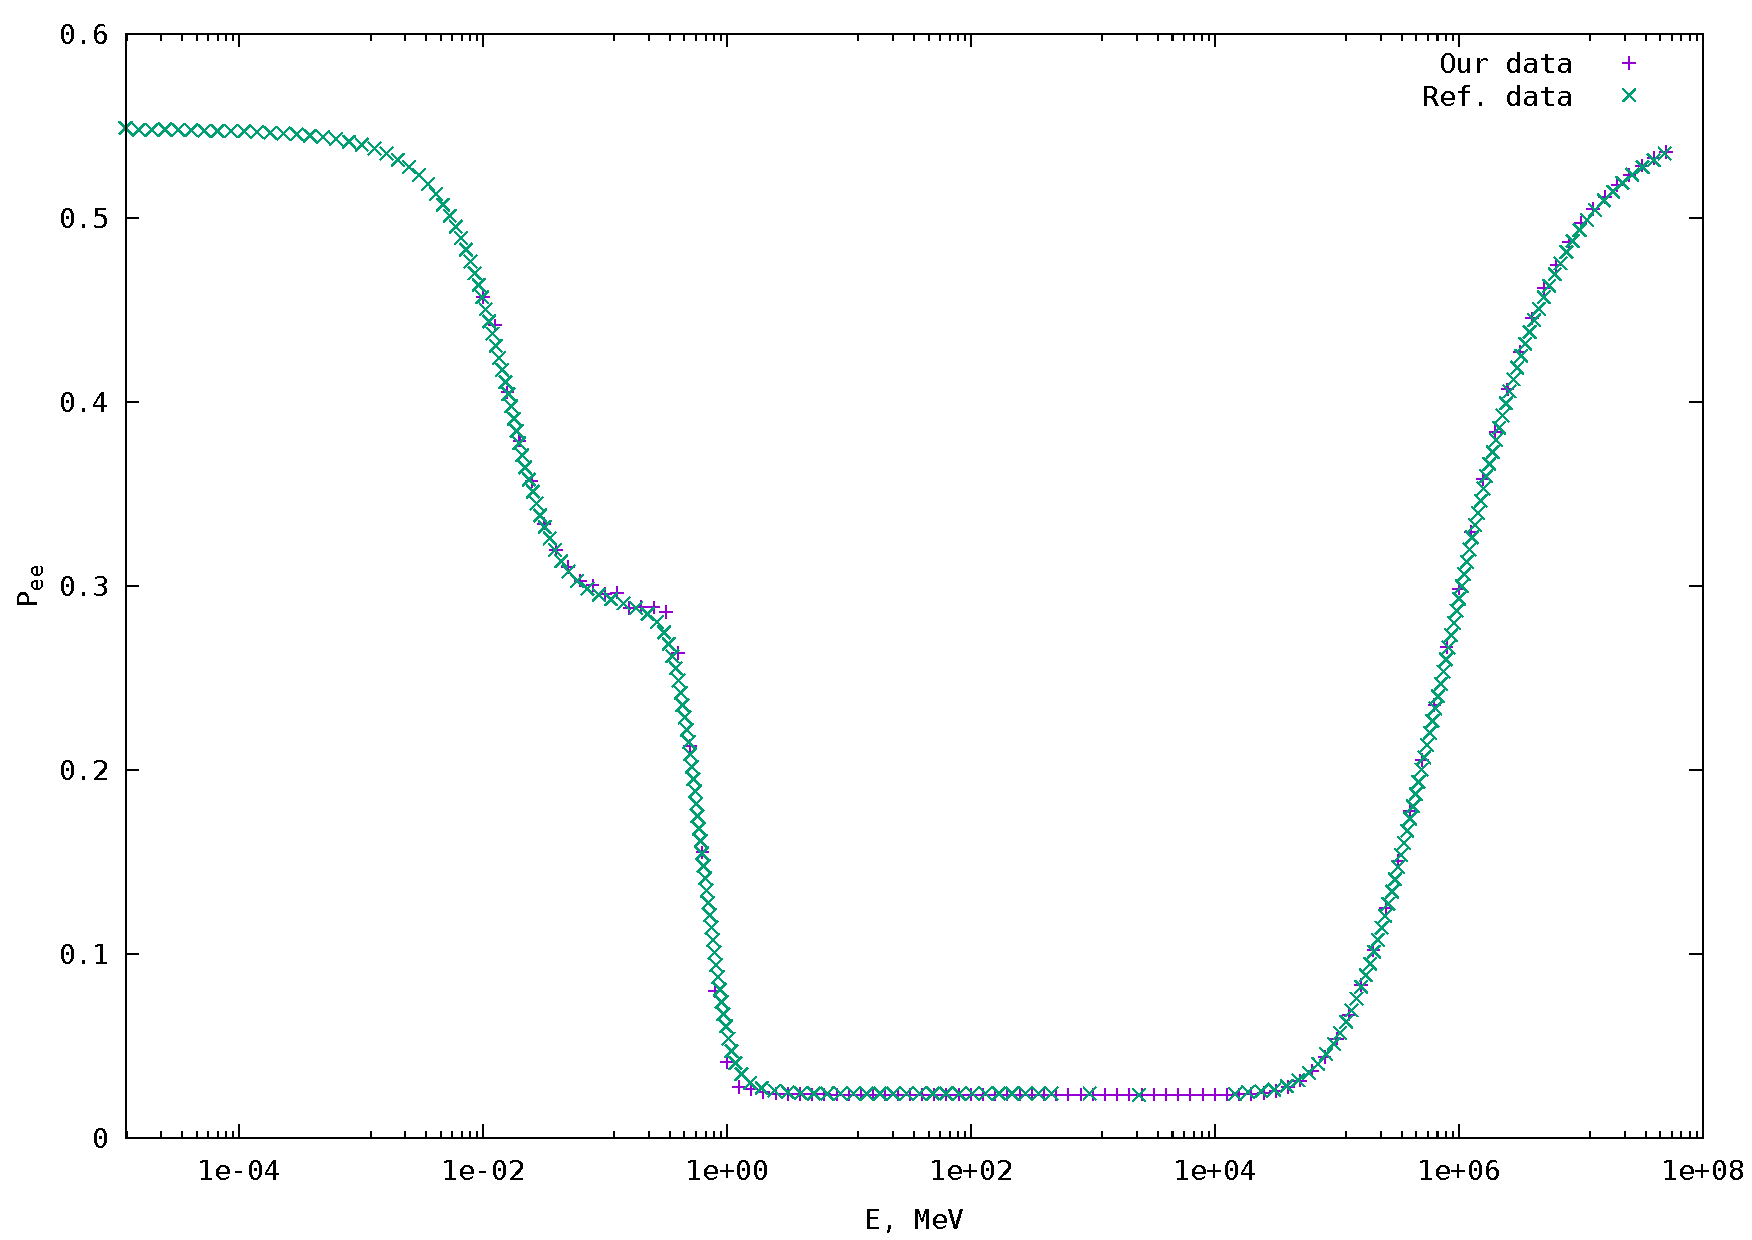
\includegraphics[scale=0.6]{sn_our_vs_ref}
  \caption{\label{fig:1}Сравнение с референсными данными для модели сверхновой.}
\end{figure}

Как видно на рис.~\ref{fig:1} наши данные очень хорошо согласуются с
референсными данными. Правда у нас мало точек при малых значениях энергии, но
это связано с тем, что при малых значениях энергии увеличивается время счёта.

Эти данные были получены при значениях параметров: \verb|tol=1e-5|,
\verb|xi=20.0|.

Интересной особенностью этой модели является поведение при малых энергиях и
малом \verb|xi|. При \verb|xi=1.0| и той же \verb|tol| имеем
\begin{figure}[htb]
  \hspace*{-2em}
%  \includegraphics[scale=0.6]{sn_our_vs_ref2}
  \caption{\label{fig:3}Сравнение с референсными данными при малом \(\xi\).}
\end{figure}

Для проверки численной точности мы провели расчёт вероятности выживания и
модулей компонент \(\Phi\) при разных значениях параметра \verb|tol|.

\begin{figure}[htb]
  \hspace*{-2em}
%  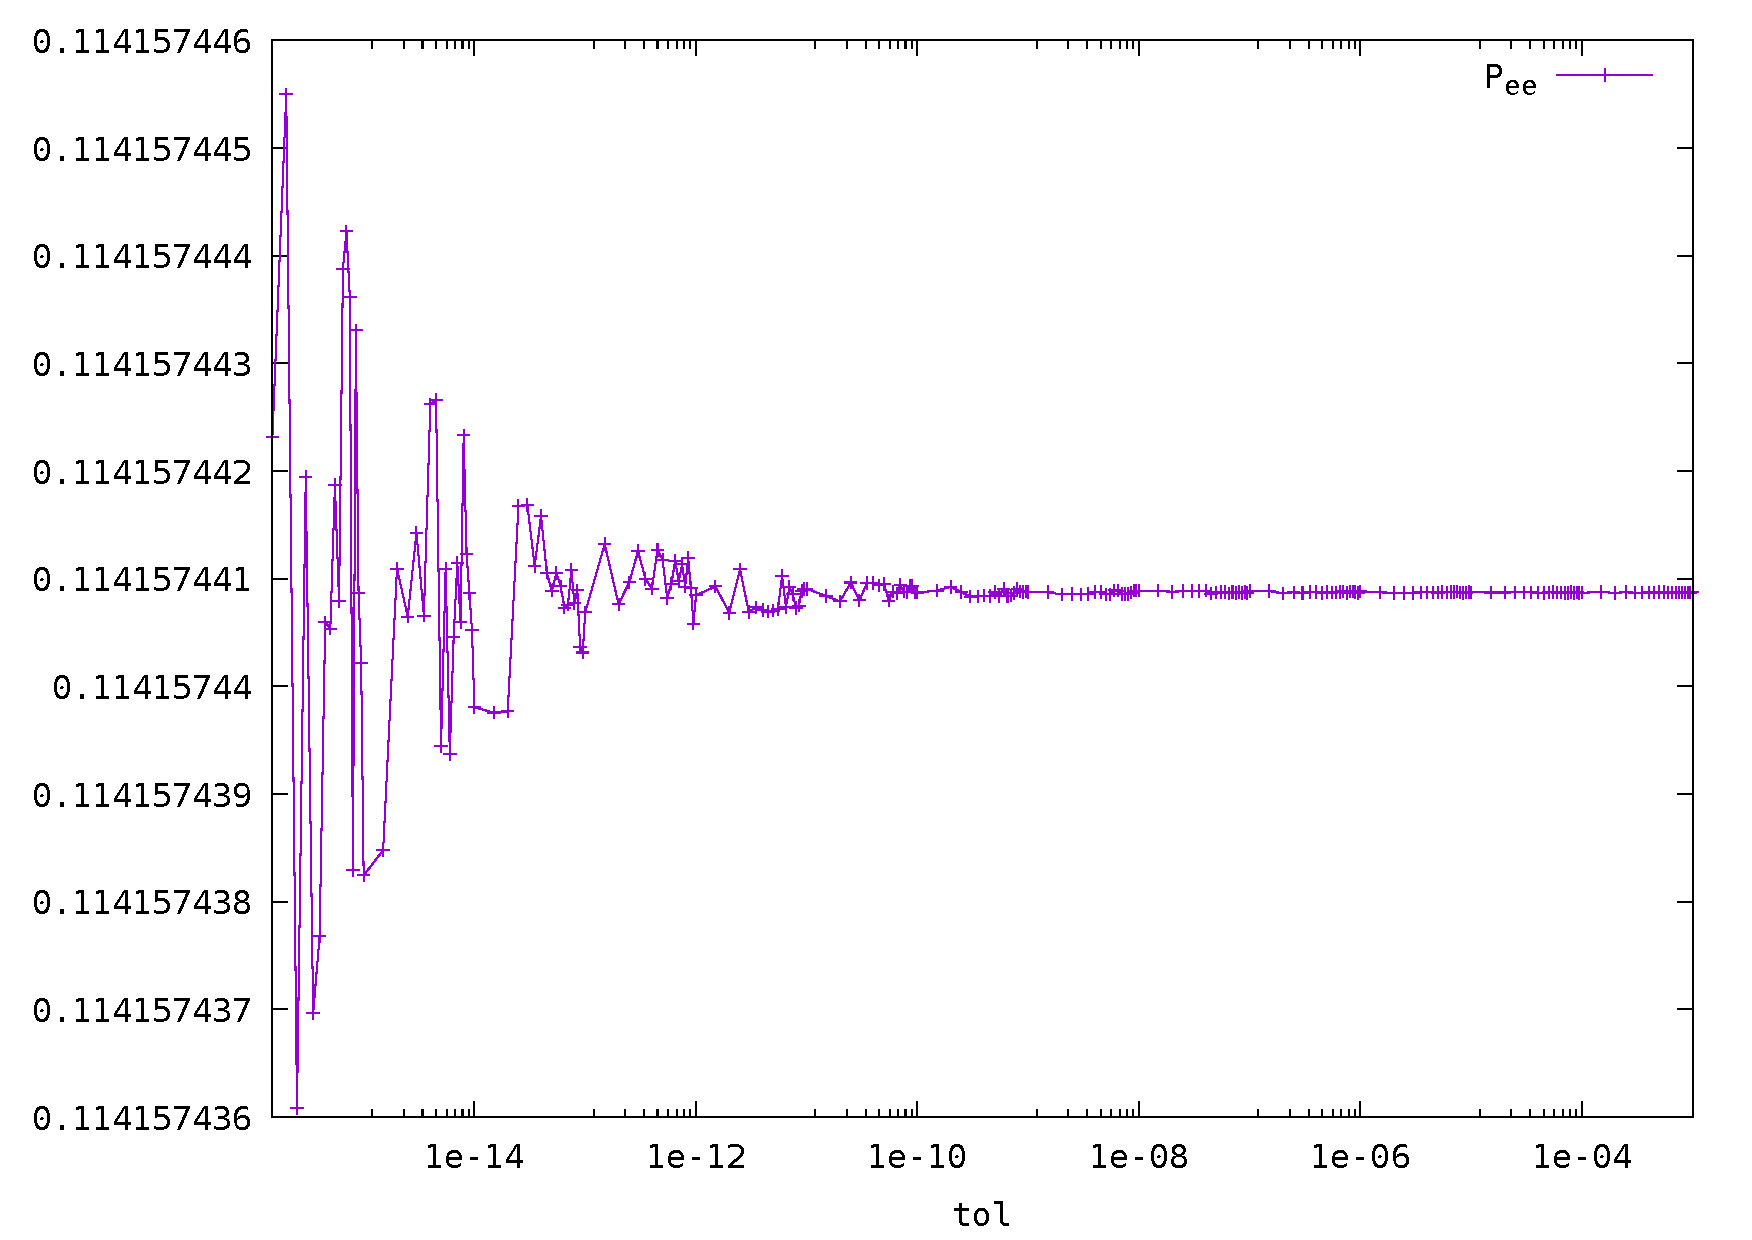
\includegraphics[scale=0.5]{sn_Pee}
  \caption{\label{fig:4}Вероятность выживания при разных \texttt{tol}.}
\end{figure}

\begin{figure}[htb]
  \hspace*{-2em}
%  \includegraphics[scale=0.5]{sn_psi1}
  \caption{\label{fig:5}Первая компоненты \(\Psi_{1}\) при разных \texttt{tol}.}
\end{figure}

\begin{figure}[htb]
  \hspace*{-2em}
%  \includegraphics[scale=0.5]{sn_psi2}
  \caption{\label{fig:6}Вторая компоненты \(\Psi_{2}\) при разных \texttt{tol}.}
\end{figure}

\begin{figure}[htb]
  \hspace*{-2em}
%  \includegraphics[scale=0.5]{sn_psi3}
  \caption{\label{fig:7}Третья компоненты \(\Psi_{3}\) при разных \texttt{tol}.}
\end{figure}

\subsubsection*{Солнечная модель}

На графике приведена вероятность выживания \(P_{\text{ee}}\) для электронного
нейтрино.
\begin{figure}[htb]
  \hspace*{-2em}
%  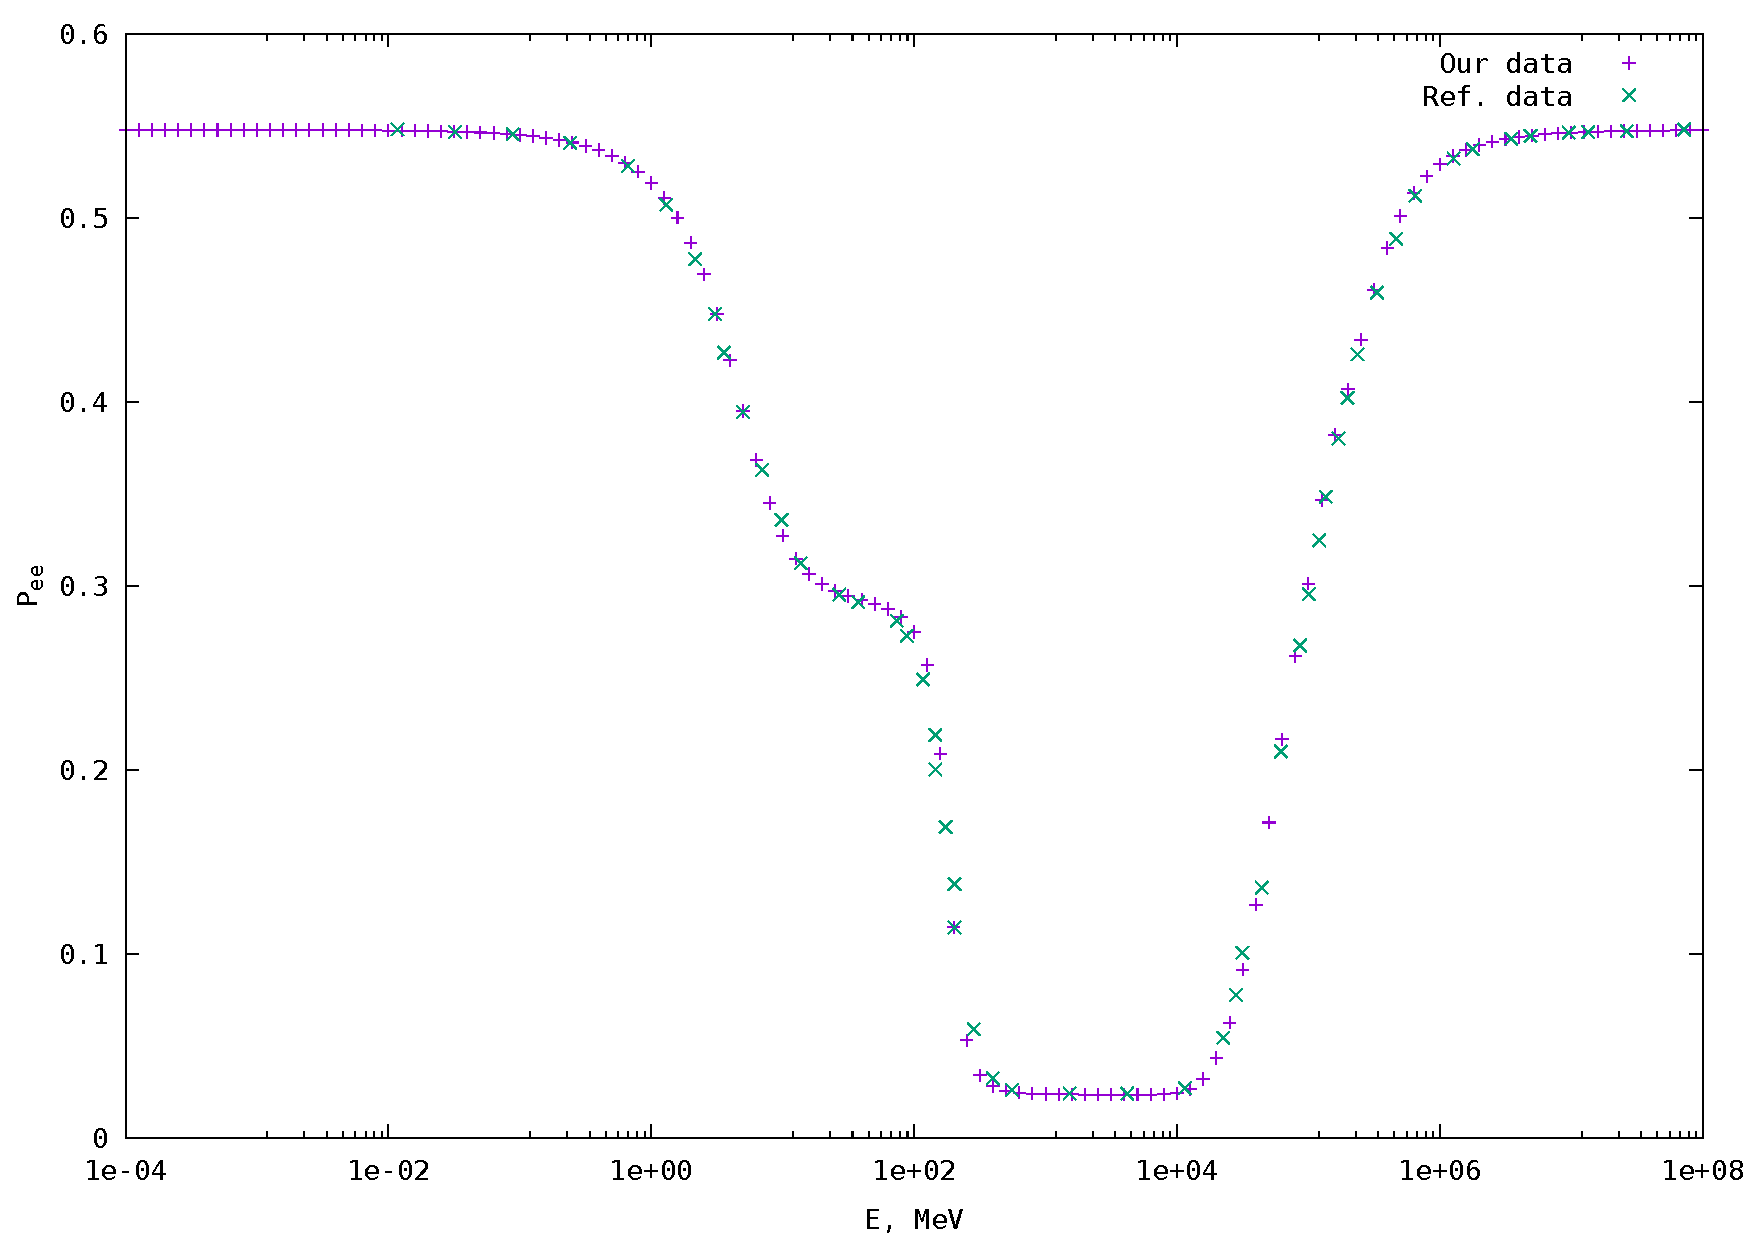
\includegraphics[scale=0.6]{sun_our_vs_ref}
  \caption{\label{fig:2}Сравнение с референсными данными для солнечной модели.}
\end{figure}

Для проверки численной точности мы провели расчёт вероятности выживания и
модулей компонент \(\Phi\) при разных значениях параметра \verb|tol|.

\begin{figure}[htb]
  \hspace*{-2em}
%  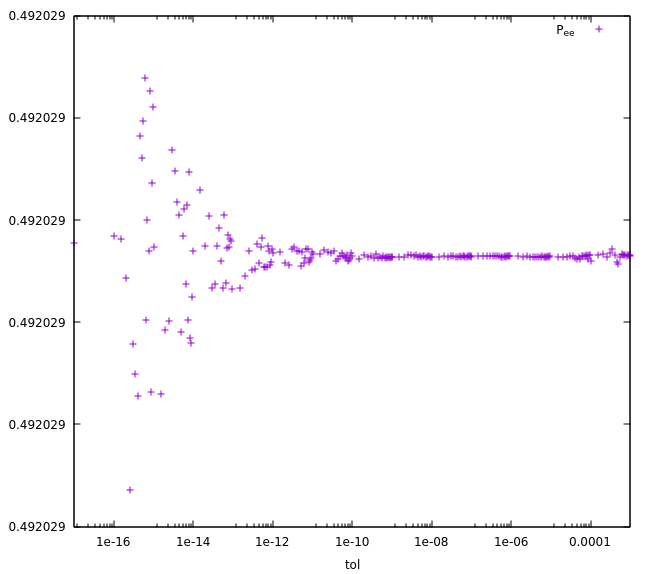
\includegraphics[scale=0.5]{sun_Pee}
  \caption{\label{fig:8}Вероятность выживания при разных \texttt{tol}.}
\end{figure}

\begin{figure}[htb]
  \hspace*{-2em}
%  \includegraphics[scale=0.5]{sun_psi1}
  \caption{\label{fig:9}Первая компоненты \(\Psi_{1}\) при разных \texttt{tol}.}
\end{figure}

\begin{figure}[htb]
  \hspace*{-2em}
%  \includegraphics[scale=0.5]{sun_psi2}
  \caption{\label{fig:10}Вторая компоненты \(\Psi_{2}\) при разных \texttt{tol}.}
\end{figure}

\begin{figure}[htb]
  \hspace*{-2em}
%  \includegraphics[scale=0.5]{sun_psi3}
  \caption{\label{fig:11}Третья компоненты \(\Psi_{3}\) при разных \texttt{tol}.}
\end{figure}

Сравнение с референсными данными показывает, что наш алгоритм работает
относительно хорошо только при больших энергиях. Несмотря на неплохое численное
поведение (см. рис. \ref{fig:9}–~\ref{fig:11}, мы имеем 6 верных знаков), он
сильно расходится при средних и малых энергиях. Нужно заметить, что в солнечной
модели профиль плотности представляет собой очень большие числа, перепад величин
от малых \(\xi\) до \(\xi=1{,}0\) достигает 4 порядков. В алгоритме есть
вычисление разности значений функции в двух близких точках, что тоже приводит к
потери точности. Несмотря на эти замечания, мы не уверены в причинах
расхождения, поэтому мы продолжим исследование причин расхождения.

\newpage
\addcontentsline{toc}{section}{\large Список литературы}
\begin{thebibliography}{99}
\bibitem{casas2016} Casas F. Efficient numerical
  integration of neutrino oscillations in matter / F.Casas, J.C. D'Olivo , J.A. Oteo // Phys. Rev. D. / F.Casas, J.C. D'Olivo, J.A. Oteo, — 2016, —
  Vol. 94, — 113008.
\bibitem{Gunti} Giunti C., Fundamentals of Neutrino Physics and Astrophysics / C. 
  Giunti, C. W. Kim. –– Oxford University Press –– 2007.
\bibitem{MSW} Wolfenstein L., Neutrino Oscillations in Matter / L. Wolfenstein, S. 
 P. Mikheyev, A. Yu. Smirnov // Phys.Rev. D. / L. Wolfenstein, S. P. Mikheyev, A. Yu. Smirnov, — 1978, — Vol. 17, — 2369-2374.
\bibitem{Magnus} A pedagogical approach to the Magnus expansion / 
 S. Blanes, et al. // Eur. J. Phys. / S. Blanes et al. — 2010, — Vol. 31, — 907–918.
\bibitem{pdg} \label{pdg} Review of Particle Physics (RPP). — URL: 
 \href{http://pdg.lbl.gov/}{http://pdg.lbl.gov/}.
\end{thebibliography}

\end{document}

%%% Local Variables:
%%% mode: latex
%%% TeX-master: t
%%% TeX-command-extra-options: "-shell-escape"
%%% End:
